\documentclass[10pt,twocolumn,oneside,a4paper]{article}
\setlength{\columnsep}{10pt}                    % Espaçamento entre colunas
\setlength{\columnseprule}{0pt}                 % Linha entre colunas (0 = sem linha)

\usepackage{amsthm}                             % Definições, teoremas
\usepackage{amssymb}
\usepackage{fontspec}                           % Configuração de fontes
\usepackage{color}
\usepackage[x11names]{xcolor}
\usepackage{listings}                           % Exibição de código
\usepackage{fancyhdr}                           % Cabeçalho e rodapé
\usepackage{graphicx}                           % Imagens
\usepackage{enumerate}
\usepackage{titlesec}
\usepackage{amsmath}
\usepackage{tikz}                               % Desenho de autômatos finitos
\usepackage{afterpage}                          % Controle de conteúdo pós-página
\usepackage{multicol}

\usepackage{amsmath, courier, listings, fancyhdr, graphicx}
\topmargin=0pt
\headsep=2pt
\textheight=790pt
\footskip=0pt
\voffset=-50pt
\textwidth=545pt
\marginparsep=0pt
\marginparwidth=0pt
\marginparpush=0pt
\oddsidemargin=0pt
\evensidemargin=0pt
\hoffset=-42pt

%%%%%%%%%%%%%%%%%%%%%%%%%%%%%

\setmainfont{Consolas}
\setmonofont{Consolas}
\XeTeXlinebreakskip = 0pt plus 1pt             % Espaçamento entre parágrafos
\setcounter{secnumdepth}{3}                    % Profundidade da numeração no sumário

%%%%%%%%%%%%%%%%%%%%%%%%%%%%%
\makeatletter
\lst@CCPutMacro\lst@ProcessOther {"2D}{\lst@ttfamily{-{}}{-{}}}
\@empty\z@\@empty
\makeatother
\lstset{                                       % Configuração de exibição de código
    language=C++,                              % Linguagem do código
    basicstyle=\footnotesize\ttfamily,         % Tamanho e fonte do código
    %numbers=left,                             % Números de linha (esquerda)
    numberstyle=\footnotesize,                 % Tamanho dos números de linha
    stepnumber=1,                              % Numeração a cada linha
    numbersep=5pt,                             % Distância número-código
    backgroundcolor=\color{white},             % Cor de fundo
    showspaces=false,                          % Mostrar espaços
    showstringspaces=false,                    % Sublinhar espaços em strings
    showtabs=false,                            % Mostrar tabs
    frame=false,                               % Moldura ao redor do código
    tabsize=2,                                 % Tamanho do tab
    captionpos=b,                              % Legenda abaixo
    breaklines=true,                           % Quebra de linha automática
    breakatwhitespace=false,                   % Quebrar apenas em espaços
    escapeinside={\%*}{*)},                    % Delimitadores para comentários no código
    morekeywords={*},                          % Palavras-chave extras
    keywordstyle=\bfseries\color{Blue1},
    commentstyle=\itshape\color{Red4},
    stringstyle=\itshape\color{Green4},
}

%----------------------------------------------------------------------------------------
%   Ajuste de espaçamento das seções
%----------------------------------------------------------------------------------------

\makeatletter
\let\origsection\section
\renewcommand\section{\@ifstar{\starsection}{\nostarsection}}

\newcommand\nostarsection[1]
{\sectionprelude\origsection{#1}\sectionpostlude}

\newcommand\starsection[1]
{\sectionprelude\origsection*{#1}\sectionpostlude}

\newcommand\sectionprelude{%
  \vspace{-10pt} % Espaço antes da seção (ajuste se quiser mais/menos)
}
\newcommand\sectionpostlude{%
  \vspace{-10pt} % Espaço depois da seção (ajuste se quiser mais/menos)
}
\makeatother

% ---------------------------------------------------------------------------------------
\usepackage{tocloft}
\cftsetindents{subsection}{1.5em}{2.5em}

% ===== CABEÇALHO E RODAPÉ =====
% ALTERE AQUI: nome da equipe e universidade
\def\NomeEquipe{Só vim pelos balões}
\def\Universidade{CEFET-MG}

\usepackage{fancyhdr}
\pagestyle{fancy}
\fancypagestyle{plain}{
    \fancyhf{}
    \fancyhead[C]{\NomeEquipe}
    \fancyhead[L]{\Universidade}
    \fancyhead[R]{\thepage}
    \renewcommand{\headrulewidth}{0.4pt}
}

\renewcommand{\headrulewidth}{0.4pt}
\renewcommand{\footrulewidth}{0pt}

\begin{document}
\pagestyle{fancy}
\fancyfoot{}
\fancyhead[C]{\NomeEquipe}
\fancyhead[L]{\Universidade}
\fancyhead[R]{\thepage}
\renewcommand{\headrulewidth}{0.4pt}
\renewcommand{\contentsname}{Sumário}           % "Contents" → "Sumário"

\textbf{
\scriptsize
\begin{multicols}{2}
  \tableofcontents
\end{multicols}
}
\newpage
%%%%%%%%%%%%%%%%%%%%%%%%%%%%%%%%%%%%%%%%%%%%%%%%%%%%%%%%%%%%%%%%%%%%%%%%%%%  BÁSICO  %%%%%%%%%%%%%%%%%%%%%%%%%%%%%%%%%%%%%%%%%%%%%%%%%%%%%%%%%%%%%%%%%%%%%%%%%%%
\setcounter{page}{1}
\section{Básico}

\subsection{Código padrão (template)}
\lstinputlisting{base/main.cpp}

\subsection{Código padrão com casos teste (template)}
\lstinputlisting{base/casos_teste.cpp}

%%%%%%%%%%%%%%%%%%%%%%%%%%%%%%%%%%%%%%%%%%%%%%%%%%%%%%%%%%%%%%%%%%%%%%%%%%%  FLUXO  %%%%%%%%%%%%%%%%%%%%%%%%%%%%%%%%%%%%%%%%%%%%%%%%%%%%%%%%%%%%%%%%%%%%%%%%%%%
\section{Fluxo e Emparelhamento}

\subsection{Dinic (fluxo máximo)}
\lstinputlisting{flow/Dicnic.cpp}

\subsection{Fluxo máximo com custo mínimo}
\lstinputlisting{flow/ZkwFlow.cpp}

\subsection{Emparelhamento Húngaro}
\lstinputlisting{flow/Hungarian.cpp}

\subsection{Kuhn-Munkres (KM)}
\lstinputlisting{flow/KM.cpp}


%%%%%%%%%%%%%%%%%%%%%%%%%%%%%%%%%%%%%%%%%%%%%%%%%%%%%%%%%%%%%%%%%%%%%%%%%%%  GRAFOS  %%%%%%%%%%%%%%%%%%%%%%%%%%%%%%%%%%%%%%%%%%%%%%%%%%%%%%%%%%%%%%%%%%%%%%%%%%%
\section{Grafos}

\subsection{Dijkstra}
\lstinputlisting{grafo/Dijkstra.cpp}

\subsection{Bellman-Ford}
\lstinputlisting{grafo/Bellman-Ford.cpp}

\subsection{SPFA}
\lstinputlisting{grafo/SPFA.cpp}

\subsection{Floyd-Warshall}
\lstinputlisting{grafo/Floyd-Warshall.cpp}

\subsection{Caminho Euleriano}
\lstinputlisting{grafo/euler.cpp}

\subsection{Componentes Biconexos (BCC)}
\lstinputlisting{grafo/BccVertex.cpp}

\subsection{Componentes Fortemente Conexos (SCC)}
\lstinputlisting{grafo/SCC.cpp}

\subsection{Clique Maximal}
\lstinputlisting{grafo/MaximalClique.cpp}

\subsection{Clique Máximo}
\lstinputlisting{grafo/MaximumClique.cpp}

\subsection{Ciclo de Média Mínima}
\lstinputlisting{grafo/Minimum Mean Cycle.cpp}

\subsection{AGM Manhattan}
\lstinputlisting{grafo/ManhattanMST.cpp}


%%%%%%%%%%%%%%%%%%%%%%%%%%%%%%%%%%%%%%%%%%%%%%%%%%%%%%%%%%%%%%%%%%%%%%%%%%%  PD  %%%%%%%%%%%%%%%%%%%%%%%%%%%%%%%%%%%%%%%%%%%%%%%%%%%%%%%%%%%%%%%%%%%%%%%%%%%
\section{Programação Dinâmica}

\subsection{PD em dígitos}
\lstinputlisting{PD/digitDP.cpp}

\subsection{SOS DP}
\lstinputlisting{PD/SOSDP.cpp}


%%%%%%%%%%%%%%%%%%%%%%%%%%%%%%%%%%%%%%%%%%%%%%%%%%%%%%%%%%%%%%%%%%%%%%%%%%%  MATEMÁTICA  %%%%%%%%%%%%%%%%%%%%%%%%%%%%%%%%%%%%%%%%%%%%%%%%%%%%%%%%%%%%%%%%%%%%%%%%%%%
\section{Matemática}

\subsection{Fórmulas}
\lstinputlisting{matematica/Formula.txt}

\subsection{Exponenciação Binária}
\lstinputlisting{matematica/expo_bin.cpp}

\subsection{Soma e multiplicação com \_\_int128}
\lstinputlisting{matematica/llladdmul.cpp}

\subsection{Primos}
\lstinputlisting{matematica/Primes.txt}

\subsection{Pares coprimos}
\lstinputlisting{matematica/coprime.cpp}

\subsection{Exponenciação rápida}
\lstinputlisting{matematica/QuickPow.cpp}

\subsection{Exponenciação rápida de matrizes}
\lstinputlisting{matematica/MatPow.cpp}

\subsection{Função totiente (φ)}
\lstinputlisting{matematica/phi.cpp}

\subsection{Tabela de fatores}
\lstinputlisting{matematica/FactorTable.cpp}

\subsection{Números de Catalan}
\lstinputlisting{matematica/CatalanNumber.cpp}

\subsection{Teste de primalidade Miller-Rabin}
\lstinputlisting{matematica/MillerRabin.cpp}

\subsection{Fatoração Pollard-Rho}
\lstinputlisting{matematica/PollardRho.cpp}

\subsection{Fatoração prima em O(log n)}
\lstinputlisting{matematica/PrimeFactorO(logn).cpp}

\subsection{Multiplicação O(1) com \_\_int128}
\lstinputlisting{matematica/O(1)mul.cpp}

\subsection{Problema de Josefo (Josephus)}
\lstinputlisting{matematica/JosephusProblem.cpp}

\subsection{Soma harmônica}
\lstinputlisting{matematica/HarmonicSum.cpp}

\subsection{Contagem de Pólya}
\lstinputlisting{matematica/Polya.cpp}

\subsection{FFT (Transformada Rápida de Fourier)}
\lstinputlisting{matematica/FFT.cpp}

\subsection{Jogo de Grundy}
\lstinputlisting{matematica/GrundyGame.cpp}

\subsection{Algoritmo de Euclides Estendido}
\lstinputlisting{matematica/Exgcd.cpp}

\subsection{Teorema Chinês do Resto (CRT)}
\lstinputlisting{matematica/CRT.cpp}


%%%%%%%%%%%%%%%%%%%%%%%%%%%%%%%%%%%%%%%%%%%%%%%%%%%%%%%%%%%%%%%%%%%%%%%%%%%  ESTRUTURAS DE DADOS  %%%%%%%%%%%%%%%%%%%%%%%%%%%%%%%%%%%%%%%%%%%%%%%%%%%%%%%%%%%%%%%%%%%%%%%%%%%
\section{Estruturas de Dados}

\subsection{PBDS (Set Indexado)}
\lstinputlisting{estruturaDeDados/PBDS.cpp}

\subsection{BIT (Fenwick Tree)}
\lstinputlisting{estruturaDeDados/BIT.cpp}

\subsection{BIT 2D}
\lstinputlisting{estruturaDeDados/BIT2D.cpp}

\subsection{Union-Find persistente}
\lstinputlisting{estruturaDeDados/persistent_dsu.cpp}

\subsection{Tabela esparsa (RMQ em O(1))}
\lstinputlisting{estruturaDeDados/Sparse Table.cpp}

\subsection{Segment Tree}
\lstinputlisting{estruturaDeDados/SegmentTree.cpp}

\subsection{Segment Tree dinâmica}
\lstinputlisting{estruturaDeDados/dinamicSegmentTree.cpp}

\subsection{Segment Tree dinâmica 2D}
\lstinputlisting{estruturaDeDados/dinamicSegmentTree2D.cpp}

\subsection{Segment Tree persistente}
\lstinputlisting{estruturaDeDados/persistent_seg_tree.cpp}

\subsection{Segment Tree temporal}
\lstinputlisting{estruturaDeDados/TimeSegmentTree.cpp}

\subsection{Treap (BST aleatória)}
\lstinputlisting{estruturaDeDados/Treap.cpp}

%%%%%%%%%%%%%%%%%%%%%%%%%%%%%%%%%%%%%%%%%%%%%%%%%%%%%%%%%%%%%%%%%%%%%%%%%%%  STRINGS  %%%%%%%%%%%%%%%%%%%%%%%%%%%%%%%%%%%%%%%%%%%%%%%%%%%%%%%%%%%%%%%%%%%%%%%%%%%
\section{Strings}

\subsection{Arranjo de Sufixos (SA)}
\lstinputlisting{string/SA.cpp}

\subsection{KMP (Knuth-Morris-Pratt)}
\lstinputlisting{string/KMP.cpp}

\subsection{Hash simples}
\lstinputlisting{string/SingleHash.cpp}

\subsection{Hash duplo}
\lstinputlisting{string/DoubleHash.cpp}

\subsection{Rabin-Karp}
\lstinputlisting{string/RabinKarp.cpp}

\subsection{Trie}
\lstinputlisting{string/Trie.cpp}

\subsection{Função Z}
\lstinputlisting{string/Zfunction.cpp}

\subsection{Rotação mínima}
\lstinputlisting{string/MinRotation.cpp}

\subsection{Manacher (palíndromos)}
\lstinputlisting{string/Manacher.cpp}

\subsection{Árvore de palíndromos (PalTree)}
\lstinputlisting{string/PalTree.cpp}

\subsection{Subsequências distintas}
\lstinputlisting{string/DistinctSubsequence.cpp}


%%%%%%%%%%%%%%%%%%%%%%%%%%%%%%%%%%%%%%%%%%%%%%%%%%%%%%%%%%%%%%%%%%%%%%%%%%%  ÁRVORES  %%%%%%%%%%%%%%%%%%%%%%%%%%%%%%%%%%%%%%%%%%%%%%%%%%%%%%%%%%%%%%%%%%%%%%%%%%%
\section{Árvores}

\subsection{LCA (Menor Ancestral Comum)}
\lstinputlisting{arvore/LCA.cpp}

\subsection{Hash de árvore}
\lstinputlisting{arvore/TreeHash.cpp}

\subsection{Decomposição Pesada-Leve (HLD)}
\lstinputlisting{arvore/heavyLightDecomposition.cpp}


%%%%%%%%%%%%%%%%%%%%%%%%%%%%%%%%%%%%%%%%%%%%%%%%%%%%%%%%%%%%%%%%%%%%%%%%%%%  GEOMETRIA  %%%%%%%%%%%%%%%%%%%%%%%%%%%%%%%%%%%%%%%%%%%%%%%%%%%%%%%%%%%%%%%%%%%%%%%%%%%
\section{Geometria}

\subsection{Definições 2D}
\lstinputlisting{geometria/2DDefinition.cpp}

\subsection{Definições 3D}
\lstinputlisting{geometria/3DDefinition.cpp}

\subsection{Definição de reta}
\lstinputlisting{geometria/LineDefinition.cpp}

\subsection{Operações básicas}
\lstinputlisting{geometria/Basic.cpp}

\subsection{Área do polígono}
\lstinputlisting{geometria/PolygonArea.cpp}

\subsection{Ponto dentro do polígono}
\lstinputlisting{geometria/IsPointInPolygon.cpp}

\subsection{Fecho convexo}
\lstinputlisting{geometria/ConvexHull.cpp}

\subsection{Soma de Minkowski}
\lstinputlisting{geometria/MinkowskiSum.cpp}

\subsection{Distância mais curta entre polígonos}
\lstinputlisting{geometria/PolygonDistance.cpp}

\subsection{Truque do fecho convexo (CHT)}
\lstinputlisting{geometria/ConvexHullTrick.cpp}

\subsection{Ordenação polar}
\lstinputlisting{geometria/PolarSort.cpp}

\subsection{Teorema de Pick}
\lstinputlisting{geometria/PickTheorm.cpp}

\subsection{Par de pontos mais próximos}
\lstinputlisting{geometria/ShortestPair.cpp}

\subsection{Par de pontos mais distantes}
\lstinputlisting{geometria/FarthestPair.cpp}

\subsection{Mediana geométrica (Weiszfeld)}
\lstinputlisting{geometria/Weiszfeld.cpp}

\subsection{Linha de varredura}
\lstinputlisting{geometria/SweepLine.cpp}

\subsection{Interseção círculo-polígono}
\lstinputlisting{geometria/CircleIntersect.cpp}

\subsection{Tangentes a dois círculos}
\lstinputlisting{geometria/TangantLineOf2Circle.cpp}

\subsection{Interseção de dois círculos}
\lstinputlisting{geometria/PCIntersect.cpp}

\subsection{Cobertura de círculo}
\lstinputlisting{geometria/CircleCover.cpp}

\subsection{Círculo mínimo envolvente}
\lstinputlisting{geometria/Mec.cpp}

\subsection{Esfera mínima envolvente}
\lstinputlisting{geometria/Mec.cpp}

\subsection{Retângulo envolvente de área mínima/máxima}
\lstinputlisting{geometria/MinMaxEnclosingRectangle.cpp}

\subsection{Interseção de semiplanos}
\lstinputlisting{geometria/HalfPlaneIntersection.cpp}

\subsection{União de polígonos}
\lstinputlisting{geometria/PolyUnion.cpp}

\subsection{Cobertura de polígonos}
\lstinputlisting{geometria/PolyCover.cpp}

\subsection{Pontos notáveis do triângulo}
\lstinputlisting{geometria/Triangle.cpp}


%%%%%%%%%%%%%%%%%%%%%%%%%%%%%%%%%%%%%%%%%%%%%%%%%%%%%%%%%%%%%%%%%%%%%%%%%%%  PROBLEMAS ESPECIAIS  %%%%%%%%%%%%%%%%%%%%%%%%%%%%%%%%%%%%%%%%%%%%%%%%%%%%%%%%%%%%%%%%%%%%%%%%%%%
\section{Problemas Especiais}

\subsection{Contagem de substrings}
\lstinputlisting{problemasEspeciais/ContainString.cpp}

\subsection{Ordem parcial 3D}
\lstinputlisting{problemasEspeciais/Partiallyordered3D.cpp}

\subsection{LCS cíclico}
\lstinputlisting{problemasEspeciais/CyclicLCS.cpp}

\subsection{Simulated Annealing (têmpera simulada)}
\lstinputlisting{problemasEspeciais/Simulated annealing.cpp}

\subsection{Raiz quadrada discreta}
\lstinputlisting{problemasEspeciais/DiscreteSqrt.cpp}


%%%%%%%%%%%%%%%%%%%%%%%%%%%%%%%%%%%%%%%%%%%%%%%%%%%%%%%%%%%%%%%%%%%%%%%%%%%  PAPEL MILIMETRADO PARA RASCUNHO  %%%%%%%%%%%%%%%%%%%%%%%%%%%%%%%%%%%%%%%%%%%%%%%%%%%%%%%%%%%%%%%%%%%%%%%%%%%
\onecolumn
\centering
\vspace{1cm}
{\large \textbf{Papel milimetrado para rascunho}}
\vspace{0.5cm}

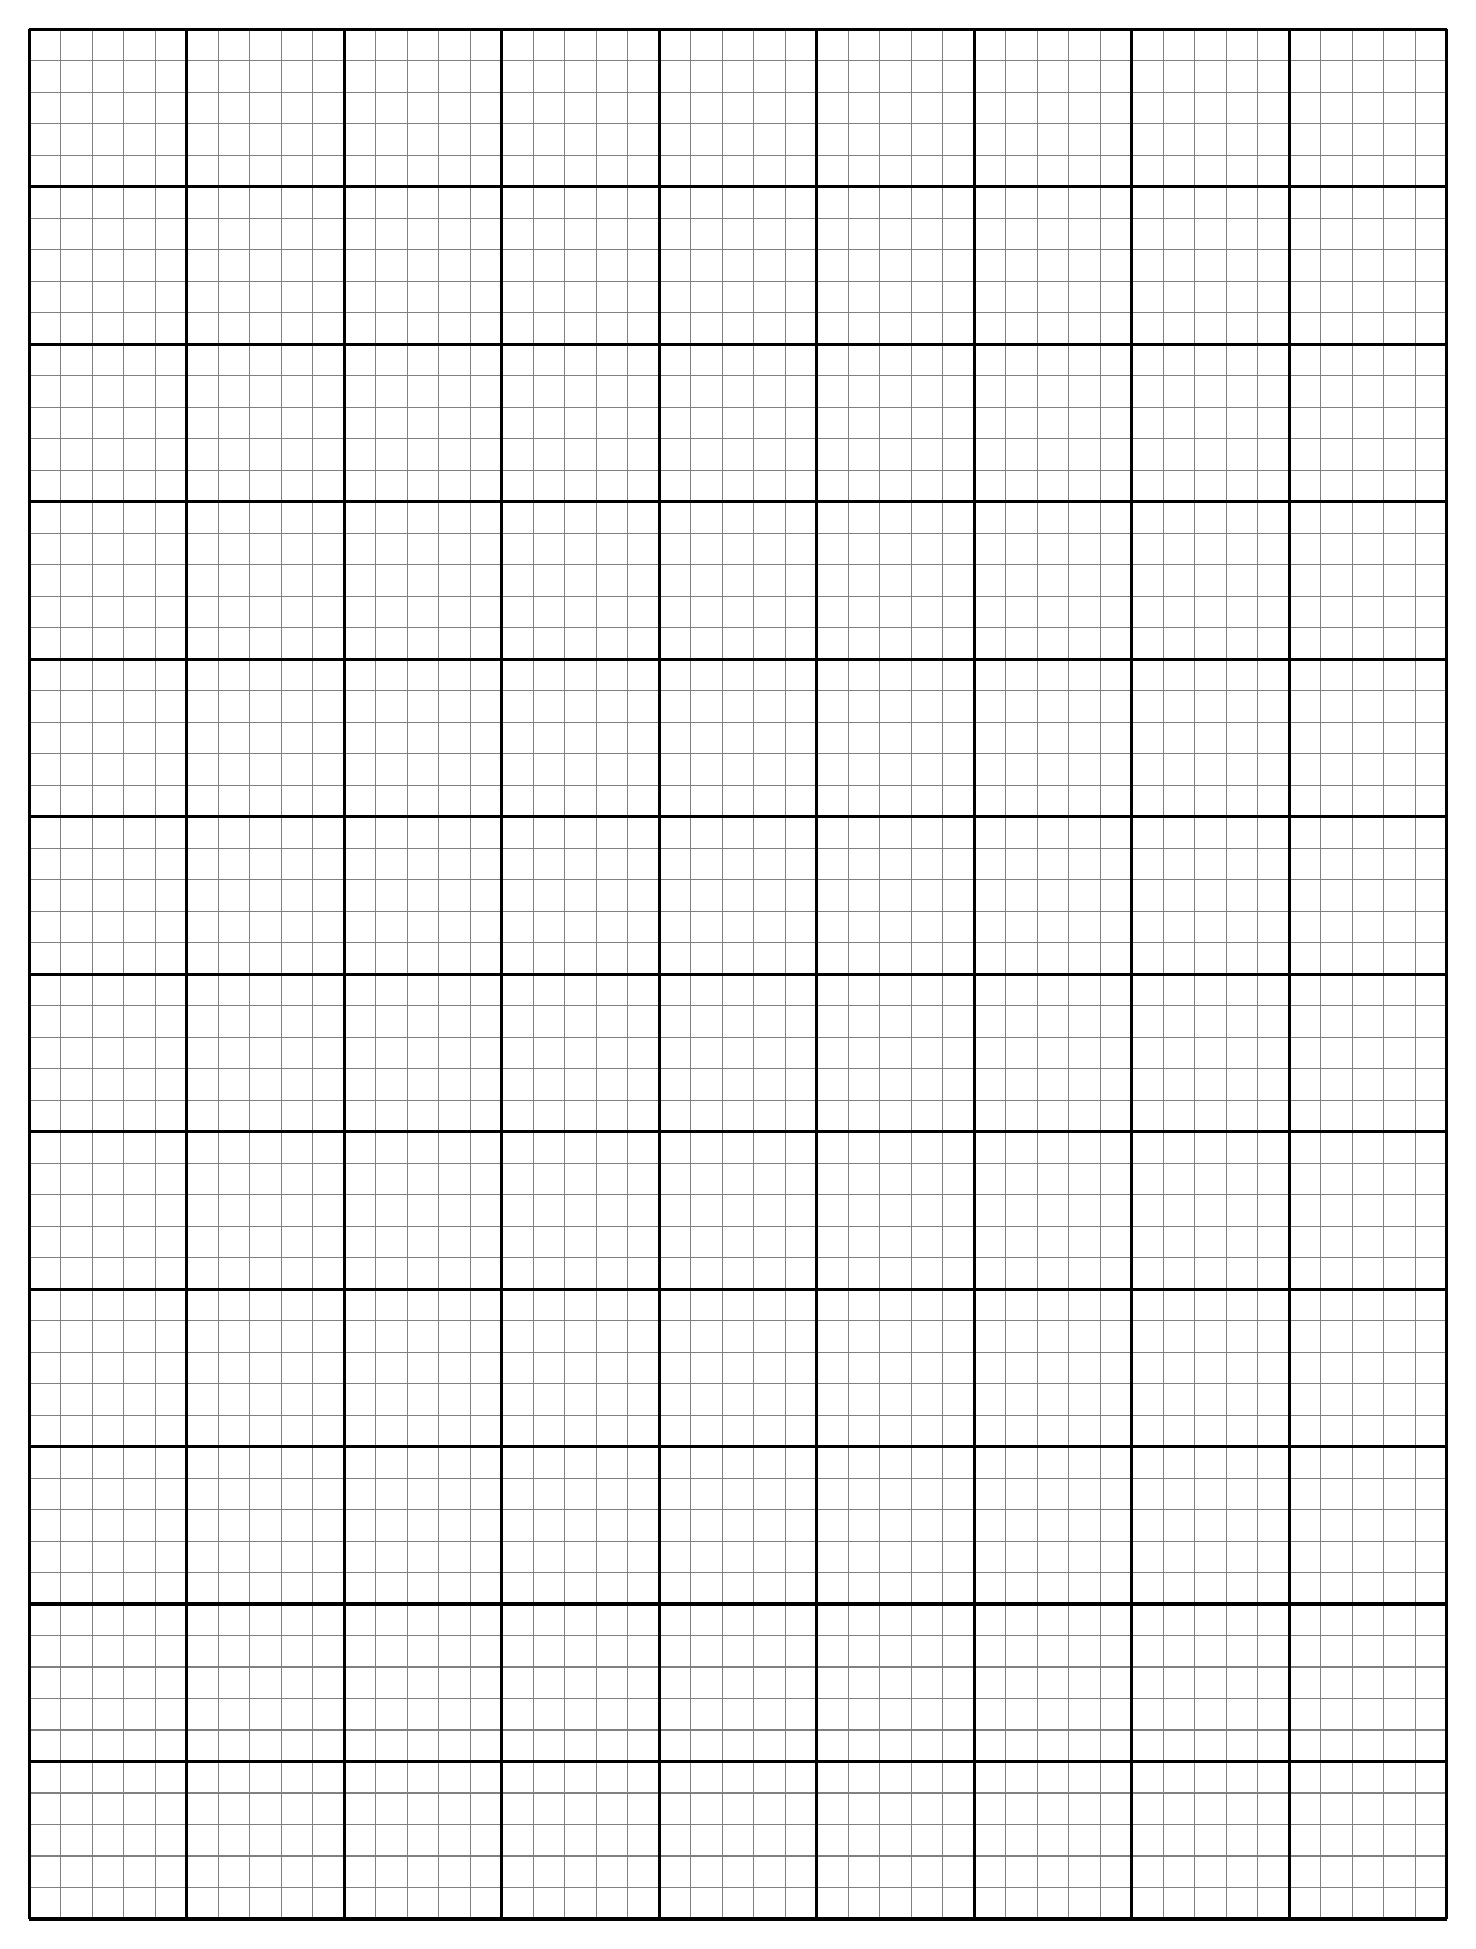
\begin{tikzpicture}[every node/.style={minimum size=1cm-\pgflinewidth, outer sep=10pt}, scale=2]
    \draw[step=0.2cm,color=gray] (0,0) grid (9,12);
    \draw[step=1cm,color=black,line width=0.4mm] (0,0) grid (9,12);
\end{tikzpicture}

\newpage

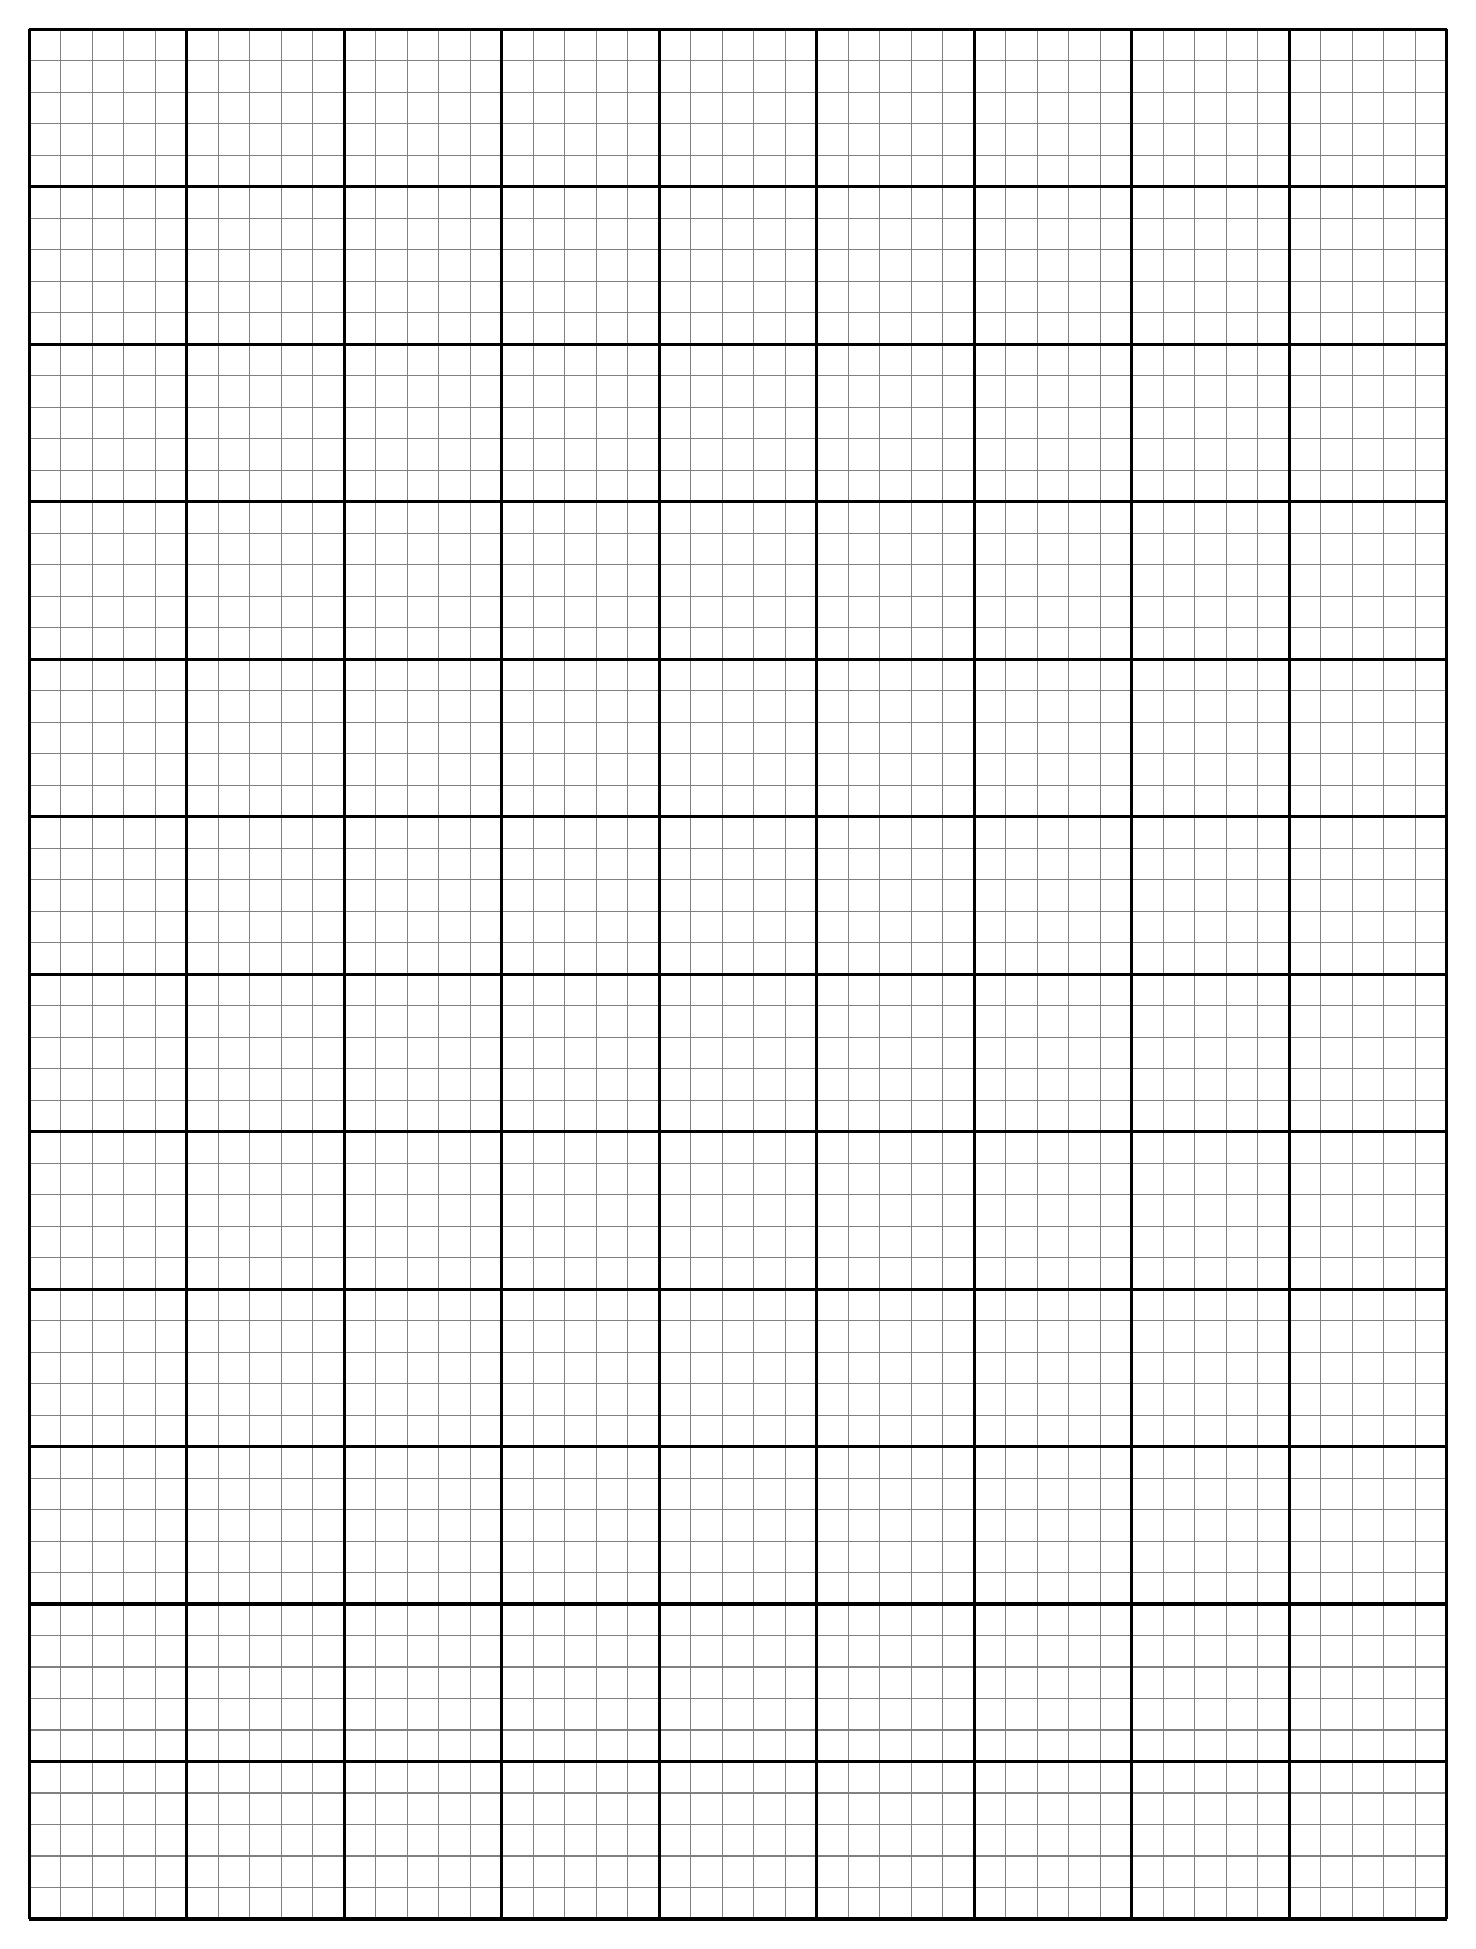
\begin{tikzpicture}[every node/.style={minimum size=1cm-\pgflinewidth, outer sep=10pt}, scale=2]
    \draw[step=0.2cm,color=gray] (0,0) grid (9,12);
    \draw[step=1cm,color=black,line width=0.4mm] (0,0) grid (9,12);
\end{tikzpicture}


\end{document}